\chapter{The Owens Valley Radio Observatory Long Wavelength Array}

\begin{bibunit}

\begin{figure}[t]
    \centering
    \begin{tabular}{cc}
        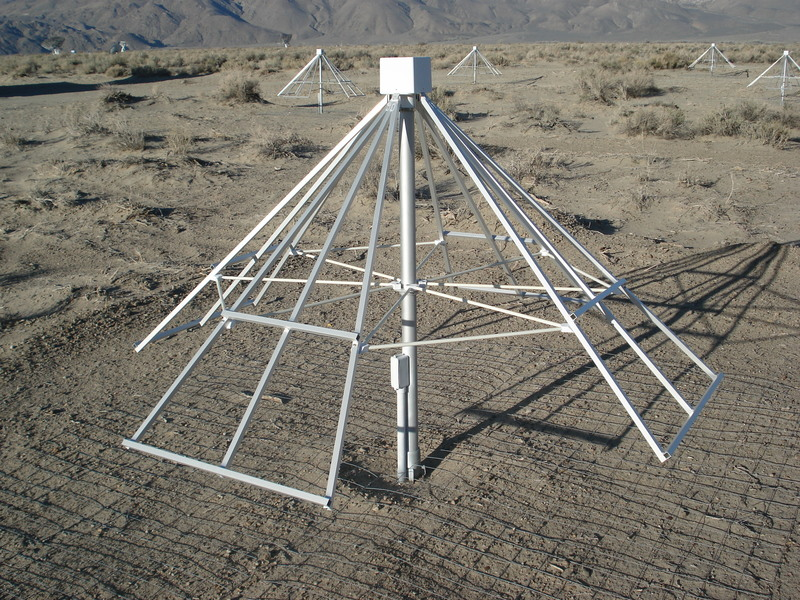
\includegraphics[height=4cm]{figures/chapter2/lwa-antenna} &
        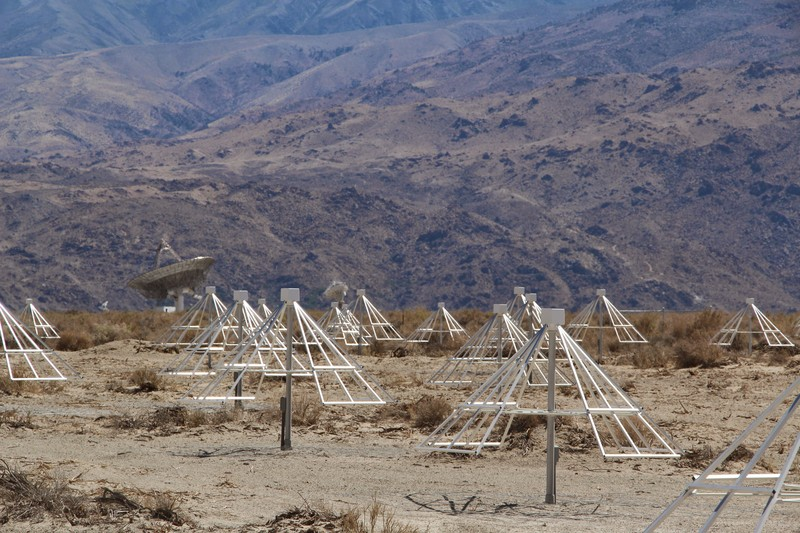
\includegraphics[height=4cm]{figures/chapter2/ovro-lwa} \\
        (a) & (b) \\
    \end{tabular}
    \caption{
        (a) A picture of an OVRO-LWA antenna.
        (b) A view of the OVRO-LWA with the Sierra Mountains in the background.
    }
    \label{fig:ovro-lwa-pictures}
\end{figure}

The Owens Valley Radio Observatory Long Wavelength Array (OVRO-LWA) is a new low-frequency radio
interferometer constructed during the course of this thesis. In its current iteration, it is
composed of 288 dual-polarization dipole antennas with a bandpass covering 27 to 85~MHz (wavelengths
between 3.5 and 11~m). 251 antennas are located with a 200~m diameter core in a pseudo-random
configuration optimized for minimum sidelobes in snapshot imaging. 32 additional antennas are
located at distances up to 1.5~km from the core of the array. At 85~MHz, the OVRO-LWA can therefore
achieve an angular resolution of 8\arcmin.

The OVRO-LWA hosts the LEDA correlator \citep{2015JAI.....450003K}, which performs full
cross-correlation of 512 input signals.


\section{The Analog Receivers}







\section{The Digital Correlator}



\section{The All-Sky Transient Monitor}

During observations, data is streamed from the LEDA correlator to the All-Sky Transient Monitor
(ASTM), which houses the compute nodes used for post-processing, imaging, and the analysis completed
in this thesis.

ASTM is composed of 10 identical nodes.\todo{Fill out specs once ASTM is back online....}





\section{Complex Gain Calibration}

The OVRO-LWA is capable of imaging the entire hemisphere in a snapshot image. This brings its own
unique calibration challenges because it is currently impossible to isolate a single compact point source
within the field of view of the interferometer.\footnote{
    Gated pulsar observations could, in principle, achieve this isolation. This capability is a key
    development area for the OVRO-LWA.
}

Many interferometers (e.g., HERA and the MWA), recognizing the difficulty of gain calibration at low
frequencies, have opted for maximally redundant antenna configurations. These configurations can
solve for many of their calibration parameters internally without relying on an incomplete sky
model, and potentially inaccurate antenna beam model. Crucially, these interferometers sacrifice
imaging fidelity, which is useful for establishing the remaining calibration parameters (e.g., the
overall bandpass cannot be solved for in an internal self-calibration routine).\footnote{
    The HERA collaboration is currently investigating the possibility of determining the overall
    bandpass through redundancies between frequency channels. The author of this thesis is not
    optimistic about this approach.
}

Detailed sky models are therefore an important calibration requirement for all low-frequency
interferometers.



Additionally, at low-frequencies there are few flux calibrators



I measured the primary beam of the OVRO-LWA in \S\ref{sec:beam}.






\begin{align}
    \b V_{ij, \text{measured}} &= \b G_i \, \b V_{ij, \text{model}} \, \b G_j^* \\
    \begin{pmatrix}
        V_{ij, \text{measured}}^{xx} & V_{ij, \text{measured}}^{xy} \\
        V_{ij, \text{measured}}^{yx} & V_{ij, \text{measured}}^{yy} \\
    \end{pmatrix} &=
    \begin{pmatrix}
        g_{i}^{xx} & g_{i}^{xy} \\
        g_{i}^{yx} & g_{i}^{yy} \\
    \end{pmatrix}
    \begin{pmatrix}
        V_{ij, \text{model}}^{xx} & V_{ij, \text{model}}^{xy} \\
        V_{ij, \text{model}}^{yx} & V_{ij, \text{model}}^{yy} \\
    \end{pmatrix}
    \begin{pmatrix}
        g_{j}^{xx} & g_{j}^{xy} \\
        g_{j}^{yx} & g_{j}^{yy} \\
    \end{pmatrix}^*
\end{align}




\begin{equation}
    \b G_i = \argmin \sum_j
        \left\|
            \b V_{ij, \text{measured}} - \b G_i \, \b V_{ij, \text{model}} \, \b G_j^*
        \right\|^2
\end{equation}

\section{Source Removal and Peeling}

Because the OVRO-LWA antenna layout is optimized for sidelobe levels in snapshot imaging, the
point-spread function (PSF) is pretty good.

\myputbib{thesis}
\end{bibunit}

